\documentclass{article}
\usepackage[margin=1in]{geometry}
\usepackage{graphicx}
\usepackage{hyperref}
\usepackage{natbib}
\usepackage{soul}
\bibliographystyle{apalike}
\usepackage{amsmath}

\title{Fish from the Sky: A Novel Framework for Capturing and Quantifying Aquatic Life via Airborne eDNA}

\author{Yin Cheong Aden Ip$^1$\textbf{*} \and
Gledis Guri$^1$\textbf{*} \and
Elizabeth Andruszkiewicz Allan$^1$ \and
Ryan P. Kelly$^1$}

\date{\today}

\begin{document}

\maketitle

\section*{}

\begin{center}
\begin{tabular}{ll}
1 & School of Marine and Environmental Affairs, University of Washington, Seattle, Washington, USA \\
\hline
\textbf{*} & shared first authorship\\
&\\
& corresponding author \textbf{adenip@uw.edu}
\end{tabular}
\end{center}

\section*{Teaser}
Aquatic life leaves traces in the air, unveiling a new frontier in passive biodiversity monitoring.

\section*{Abstract}
When droughts, floods, or contamination events render water sampling unsafe or impossible, managers lose critical visibility and vital insights into aquatic ecosystems. Here, we demonstrate for the first time that aquatic life can be not only detected, but reliably quantified from the air, creating a new biomonitoring pathway. Despite advances in environmental DNA (eDNA) methods, water and air have been treated as separate genetic reservoirs and assumed to have negligible exchange. We hypothesized that natural processes such as evaporation, aerosolization, and splashing, can transfer genetic material from water into the atmosphere as airborne eDNA. We tested this at a Coho salmon (\textit{Oncorhynchus kisutch}) spawning stream by deploying four simple air samplers—gelatin, PTFE, and MCE filters, plus an open tray of deionized water—alongside paired water samples and visual counts over a six-week peak run. We then quantified eDNA concentrations in both air and water  (air: copies/day/cm²; water: copies/L) using quantitative PCR. Airborne fish eDNA concentrations were roughly 10 billion times lower than in water, yet two air collection types (PTFE and gelatin filters) tracked salmon density in near real time, mirroring both water-eDNA levels and visual counts. In contrast, the other two air collection types (MCE filters and the water tray) diverged from the water-eDNA levels and visual counts, highlighting recovery biases likely due to sampler material, orientation, and particle size. This proof-of-concept demonstrates the air–water interface is a quantifiable reservoir of aquatic genetic information, establishing airborne eDNA as a novel and low-impact proxy for aquatic population monitoring. In an era of hydrological extremes and public-health risks, airborne eDNA offers resilient pathways for opening new frontiers for conservation, resource management, and public-health protection.

%Aquatic life can now be identified and quantified from the air. Here we demonstrate, for the first time, that genetic material from water medium is transported into the atmosphere (in form of airborne genetic material, environmental DNA --  eDNA) via natural processes like evaporation, aerosolization, and splashing. Despite ongoing advancements in eDNA sampling techniques, water and air have been conceptualized as distinct genetic repositories, with previous research assuming negligible DNA exchange between these mediums and thus sampling them independently to assess biological activity in each environment. We tested this assumption by evaluating four passive airborne eDNA collection methodologies -- three different air filters (gelatin, PTFE, and MCE) and an open container of deionized water -- at one salmon spawning stream. Using qPCR, we quantified coho salmon (\textit{Oncorhynchus kisutch}) air eDNA concentration (copies/day/cm$^2$) and compared it against conventional water-based eDNA qPCR measurements (copies/L) and direct visual fish counts (fish/day) to determine which air-sampling approach most accurately reflected fish density. We found that air eDNA concentration is approximately 10 orders of magnitude lower than water concentration ($\eta \approx e^{-10}$ units: $\frac{copies/day/cm^2}{copies/L}$). Among the collection methods, PTFE and gelatin air filters most closely correlated with fish signals obtained from water sampling and visual counting, while MCE air filters and the deionized water container exhibited different patterns. This research represents a paradigm shift by identifying air as a previously unrecognized repository of aquatic genetic information, establishing airborne eDNA as a novel and valuable proxy for monitoring aquatic biological activity and population dynamics. This framework opens new frontiers for environmental genomics, conservation biology, ecosystem and public health management in a rapidly changing world.\\


\textbf{Keywords}: environmental DNA, Air eDNA, Passive Air Filtration, Aquatic Biomonitoring, Aerosolization, Evaporation, Non-invasive Sampling, Quantitative eDNA Analysis, Salmon, Environmental Genomics

\section{Introduction}
Monitoring aquatic life is fundamental to understanding ecosystem health, guiding conservation efforts, and managing valuable natural resources (Dudgeon et al., 2006; Reid et al., 2019). Traditional surveys, including direct visual counts, quadrat survey diving, baited remote underwater video (BRUV), acoustic trawling, netting, and trapping, have long served as the backbone of aquatic monitoring (Guri et al., 2024). Although these methods provide valuable data, they often present logistical challenges, resource limitations, and potential disturbance to sensitive aquatic communities (Guri et al., 2024).

Over the past decade, environmental DNA (eDNA) has upended our paradigm for biodiversity assessment by detecting organisms through the genetic material they shed into their surroundings. Water-based eDNA surveys are becoming a mainstream biomonitoring tool, consistently demonstrating remarkable efficacy in species detection and abundance quantification (Altermatt et al., 2025). These approaches have proven particularly effective for monitoring endangered species (Biggs et al., 2015), early detection of invasive species incursions (Thomas et al., 2020), characterizing community composition (Wilkinson et al., 2024), and even providing quantitative assessments for complementing traditional surveys (Allan et al., 2023; Guri et al., 2024; Tillotson et al., 2018). Advances in sampling protocols, laboratory workflows, and bioinformatic analyses have driven sensitivity and taxonomic resolution to new heights (Altermatt et al., 2025). Yet, all these methods remain water-centric, requiring direct water access, and often requiring specialized gear and cold-chain logistics (Spens et al., 2017; Deiner et al., 2017). These requirements become constraints during extreme hydrological events—when droughts parch rivers, floods render wading unsafe, or public-health concerns close off contaminated waters— and even eDNA surveys cannot be conducted in waterways during these events (Chen et al., 2024; Ruiz‐Ramos et al., 2023; Wan et al., 2023).

Although water-based methods are impossible under these extreme conditions, the thin layer of air immediately above rivers and lakes, where water, heat, and particles continually exchange, remain an untapped dimension of biomonitoring. While, airborne eDNA research has emerged as a promising frontier, research has  focused on detecting terrestrial organisms in a non-quantitative manner (Klepke et al. 2022; Lynggaard et al. 2023, Johnson et al., 2024). Both active and passive air filtration methods have been shown to recover DNA from mammals, birds, insects, and plants under field and enclosed conditions (Clare et al., 2021; Garrett et al., 2023; Johnson et al., 2019; Johnson et al., 2023; Lynggaard et al., 2022; Lynggaard et al., 2024; Roger et al., 2022). These air-sampling techniques sometimes detect aquatic taxa, but they are never the focus of the study and are often cited as suspected contamination or attributed to zoo feed or piscivores fecal bioaerosols (Klepke et al., 2022; Lynggaard et al., 2022; Lynggaard et al., 2023; Sullivan et al., 2023), rather than recognized as a genuine ecological signal (Tournayre et al., 2025). 

Aquatic species signals detected in air samples represent an unexplored, rich, untapped source of data for an even lower impact biodiversity monitoring method. Despite these parallel advances in aquatic and airborne eDNA research, the question of whether aquatic genetic material can naturally transfer across media into the air remains untested. Without systematic investigation, these "unexpected" aquatic signals in airborne eDNA data are often overlooked, resulting in an oversight that risks discarding a potentially powerful biomonitoring tool, especially in the face of environmental changes when water access can become unreliable or unsafe.

Environmental systems are inherently interconnected (Folke et al., 2021), and basic physics points to why aquatic DNA should appear in air (Monahan et al., 1986; Seinfield and Pandis, 2016). Natural physical processes at the air-water interface, such as evaporation, bubble-burst aerosolization from riffles and splashes, and leaping fish, churning substrates, create splash-driven aerosols; all of these provide plausible mechanisms for transferring eDNA into the atmosphere (Duchemin et al., 2002; Mueller et al., 2008; Stell et al., 2019; Van Dijk et al., 2003). These potential mechanisms would suggest that air could act as a diluted, but still informative, extension of the aquatic environment, representing biological signals that are real, quantifiable, and ecologically meaningful.

To test this hypothesis, we conducted the first targeted investigation of cross-medium water-to-air eDNA transfer, specifically examining whether genetic material from aquatic organisms can be detected in air samples collected above water surfaces. Leveraging the behavior of Coho salmon (\textbackslash{}textit\{Oncorhynchus kisutch\}) during their spawning season (Mueller et al., 2008), we collected and measured eDNA concentrations in paired water and passive air samples over a six-week peak migration period, with visual fish counts from hatchery staff. To evaluate the mechanisms of airborne DNA capture and settlement, we deployed four passive air collection methods: vertically orientated gelatin air filters (commonly used in low-flow air filtration systems), polytetrafluoroethylene filters (PTFE; standard in high-flow air applications), and mixed cellulose ester filters (MCE; traditionally employed for water filtration), as well as an open, horizontal tray of deionized water exposed to ambient conditions. These were chosen for their distinct physical properties, contrasting orientations, and different particle capture efficiencies targeting different aerosol types. By comparing detection sensitivity, quantitative capabilities, and temporal patterns of these four collection methods against water-derived eDNA concentrations and fish counts, we asked whether airborne eDNA realistically reflects real-world aquatic population dynamics.

Our findings provide the first quantitative evidence that aquatic genetic material can indeed transfer from water to air under natural conditions, and extends further with quantitative demonstrations that reflect actual population dynamics with just passive air samplers. This cross-medium detection and quantification represents not merely a technical advancement, but a conceptual leap in ecological monitoring: the previously ignored air–water interface now emerges as a measurable reservoir of aquatic genetic information. While this study centers on salmon, its implications extend broadly, proving that aquatic eDNA in the air is quantifiable and potentially species rich. This advancement re-imagines ecological monitoring as one that bridges water and air to build more resilient, comprehensive surveillance networks in a rapidly changing world.


%We also establish, for the first time, a quantitative link between airborne DNA concentrations and underlying aquatic species abundance using statistical modeling. Together, these findings represent a conceptual leap, demonstrating that aquatic life can be tracked through the air and that these signals quantitatively reflect real-world population trends. This opens the door to robust, real-time ecological inference from the atmosphere. In the absence of validated methods and models, the utility of airborne eDNA for aquatic systems has remained speculative. Addressing this gap is essential to develop a truly low-impact, scalable, and continuous monitoring framework capable of operating where conventional techniques fall short.

%The primary objective of this study is not merely to validate passive airborne sampling, but to introduce a novel framework for capturing aquatic eDNA from the air. By drawing on principles from airborne particulate filtration and repurposing materials commonly used in air microbiology, we systematically evaluated whether environmental DNA from aquatic systems can be collected passively through gravitational settling. We proposed and tested a range of varying sampling materials, PTFE, gelatin, MCE filters, and an open container of water as a particle settlement collector; chosen for their distinct physical properties and hypothesized affinities for settling DNA particles. By integrating these designs with the “air is dilute water” hypothesis, we demonstrate a conceptual and technical advance in how aquatic eDNA can be detected and quantified in air. The resulting approach offers substantial advantages in safety, and scalability, opening a new frontier for non-invasive, real-time biomonitoring. Although the study focuses on salmon, the broader potential of this framework extends to a wide range of aquatic organisms. The findings not only can simplify field operations by reducing logistical demands and operational risks but more importantly reveal that ecological signals are not confined to water bodies. Rather, the air can serve as an additional, quantifiable reservoir of biodiversity data. Collectively, these results lay the groundwork for transforming ecological monitoring into a more comprehensive, real-time process capable of improving resource management in rapidly changing environments.

\begin{figure}[tbhp] 
\centering
\includegraphics[width=13.5cm]{Figure1_new.png}  
\caption{(A) Conceptual illustration of how aquatic environmental DNA (eDNA) is transported from water into the atmosphere and subsequently captured by passive sampling devices. Natural processes, including evaporation, aerosolization, and splashing, transfer trace amounts of eDNA from a river ecosystem into the air, where four passive airborne particle collectors recover the DNA molecules as it settles. Arrows highlight the movement of DNA-containing droplets from water to air and into sampling devices. (B) Field deployment of the open container and air filters along a hatchery railing. The tray of water is visible at the lower right. (C) The air filters (PTFE, gelatin, and MCE) are hung approximately 30 cm below, and are positioned beside the open water container, about 3 m above the water’s surface. This configuration minimizes splash contamination and captures airborne DNA particles driven by gravitational settling. The positioning relative to flowing water demonstrates how these passive collectors operate at a vantage point above the stream, facilitating non-invasive DNA capture in real-world field conditions.}
\label{fig:AI_physical_model}
\end{figure}

\section{Methods}

\subsection{Field Sampling}

The study was conducted in Issaquah Creek, a salmon spawning stream, outside of the Issaquah Salmon Hatchery (47.529501$^\circ$ N, 122.039133$^\circ$ W) from 26 August 2024 to 18 November 2024, with nine sampling trips. Given our focus on coho salmon (\textit{Oncorhynchus kisutch}) and our knowledge of their spawning window (peak abundance observed from 17 October 2024 onward), sampling was strategically timed to capture the lowest to highest levels of eDNA release. Visual counts were performed by hatchery staff, and salmon escapement data were obtained from the Washington Department of Fish and Wildlife escapement reports (\href{https://wdfw.wa.gov/fishing/management/hatcheries/escapement#2024-weekly}{https://wdfw.wa.gov/fishing/management/hatcheries/escapement\#2024-weekly}). Environmental conditions varied across sampling events, ranging from fair weather to heavy rain (see Supplementary Material 1 for detailed meteorological records).

Sampling was conducted in 24-hour blocks with deployment and recovery around 9 a.m. (river water was collected only on the first day/timepoint). Four passive collection methods were evaluated: three filter types—gelatin (Sartorius, 47 mm diameter), PTFE (Whatman, 47 mm diameter), and MCE (Sterlitech, 5.0 $\mu$m pore size, 45mm diameter)—and an open container of deionized water. The rationale for selecting these materials is as follows: PTFE filters are noted for their high durability and are widely used in active air sampling experiments (Harnpicharnchai et al., 2023); gelatin filters are effective at capturing airborne particles and are particularly suited for applications where maintaining viability (e.g., for subsequent bacterial culturing; Wu et al., 2010) is desired; whereas MCE filters, typically employed for water filtration, were included to assess their performance in an airborne context (Allan et al., 2023). All three passive filters were deployed via custom 3D-printed filter holders (source code REF) and were suspended from a hatchery railing approximately 3 m above the river water level (Figure \ref{fig:AI_physical_model}), with their collection surfaces oriented horizontally. Two biological replicates were deployed for both gelatin and PTFE, while only one replicate was used for MCE. After the overnight deployment, filters were carefully recovered using sterile, disposable forceps and immediately immersed in 1.5 mL of DNA/RNA Shield. 

The fourth passive collection method was an open container (25 cm width, 30 cm length, 10 cm depth) filled with 2 L of deionized water also positioned about 3 m above the river and about 30 cm below the suspended passive filters. The open container was also deployed for about 24 hours at the same times as the passive filters. The container had an open surface (i.e., oriented horizontally) to capture airborne particles settling by gravity. The surface area of the container was approximately 750 cm$^2$, in contrast to the roughly 16 cm$^2$ surface area offered by the 47-mm circular filter disks. Only one replicate was used for the open water container method. Note that although 2 L of deionized water was placed in the container, heavy rainfall during overnight deployments sometimes increased the water level. Any debris (e.g., bugs, leaves) was removed from the container before on-site filtration using the same system as for river water samples (see below for details).

Concurrent with airborne sampling, water samples were collected by hand from the river directly adjacent to the coho salmon aggregation school, just downstream of the fish ladder entrance. A total of 3 L of water was filtered on site using a Smith-Root Citizen Science Sampler equipped with 5.0 µm mixed cellulose ester (MCE) filters (Allan et al., 2023). Three 1 L replicates were processed and immediately preserved in 1.5 mL of DNA/RNA Shield (Zymo Research) using clean disposable plastic forceps. Field-negative filtration blanks (1 L of Milli-Q water each) were also processed using the same system. All equipment was decontaminated with 10\% bleach, thoroughly rinsed with deionized water, and handled with gloves to minimize contamination. All filters (passive air, passive open container, water) were stored at –20$^\circ$C until processing, typically within one week.


\subsection{Wet-Laboratory Procedures}
DNA extraction from both river water samples and airborne filter samples was performed using the Qiagen Blood and Tissue Kit according to the manufacturer’s protocols. During extraction, it was noted that the gelatin filters dissolved completely in the DNA/RNA Shield. Samples were vortexed for 1 minute, and 500 $\mu$L of the shield was used for DNA extraction.

qPCR assays targeted a 114-bp fragment of the cytochrome b gene of coho salmon, using primers derived from Duda et al. (2021)— COCytb\_980-1093 Forward: CCTTGGTGGCGGATATACTTATCTTA and COCytb\_980-1093 Reverse: GAACTAGGAAGATGGCGAAGTAGATC. SYBR Green chemistry was employed using SYBR Select Master Mix (Fisher Scientific) on an Applied Biosystems QuantStudio 5 real-time PCR system with a 384-well block. Each 10 $\mu$L reaction consisted of 5 $\mu$L of SYBR Select Master Mix, 0.4$\mu$L of 10 mM forward primer, 0.4 $\mu$L of 10 mM reverse primer, 2.2 $\mu$L of molecular grade water, and 2 $\mu$L of DNA template. Melt curve analysis was performed to confirm the amplification of the target fragment, with an accepted melting temperature of 81$^\circ$C ± 1$^\circ$C.

Standard curves were constructed using a coho tissue DNA extract quantified with a Qubit fluorometer. The stock solution was diluted to 1.0 ng/$\mu$L and designated as 106 copies/$\mu$L. Serial dilutions were then prepared, with 105, 104, and 103 copies/$\mu$L run in triplicate, 102 copies/$\mu$L in quadruplicate, and 101/$\mu$L copies in triplicate.


\subsection{Bayesian model}
\subsubsection{Visual observation model}
We model the upstream migration of coho salmon (\textit{Oncorhynchus kisutch}), during which individuals accumulate at a river dam (hatchery). The hatchery crew periodically opens the dam gate at time $i$ to allow passage. Between successive gate-opening events ($\Delta i$), coho salmon accumulate. Let $X$ represent the true daily accumulation rate (also fish density at the river dam) in units of fish/day at time $i$, and E denote the number of days elapsed between consecutive gate openings ($ E_i =\Delta i; E_{i=1} = 0$). Prior to each gate opening (at time \textit{i}), the crew conducts a visual count $N_i$ of accumulated fish.
Assuming $X_i$ remains relatively constant between successive gate-opening events ($\Delta i$), we model the observed fish counts as a Poisson process:
\begin{equation}
\lambda_i = X_i \cdot E_i \\
\end{equation}

\begin{equation}
N_i \sim \mathrm{Poisson}(\lambda_i)
\end{equation}

where, $\lambda_i$ represents the expected number of fish accumulated over the $E_i$-day interval.

\subsubsection{Molecular (water and air) observation model}
Let $W$ be the unobserved eDNA concentration (copies/$\mu$L) in the water at time $i$ and let $\omega$ be the ``integrated eDNA factor" -- the conversion factor between $X$ and $W$ (see \cite{guri2024a} for further interpretation of this parameter). We can express the relation between the fish density and water eDNA concentration as:
\begin{equation}
X_{i} = W_{i} \cdot \omega
\end{equation}

Let $A$ be the unobserved eDNA concentration (copies/$\mu$L) in the air at time $i$ that is filtered using passive filter $j$. We model the air eDNA concentration as a function of aerosolization of the water DNA through a log-linear function with intercept $\eta$, slope = 1, and error term $\varepsilon$ (variability; time and filter specific):

\begin{equation}
\ln(A_{ij}) = \eta_{j} + \ln(W_{i}) + \varepsilon_{ij}
\end{equation}

Here the intercept $\eta$ can be interpreted as the aerosolization (or dilution from water to air) factor and error term $\varepsilon$ as parameter of the sum of squares error (SEE) from a linear regression where $\varepsilon_{ij} \sim \mathcal{N}(0,\tau_j)$.

For some filter types $j$ (PTFE filters (${j=P})$; gelatin filters (${j=G}$)) we sampled two biological replicates and we used the mean of those biological replicates to determine the average concentration in the air $A$ at time $i$ as following:

\begin{equation}
%A_{ij} = \frac{1}{B} \cdot \sum_{b=1}^{B} A_{ijb}
A_{ij} = A_{ijb} + \delta_{ijb} \qquad \text{for} \ j \in \{P,G\}
\end{equation}

%\begin{equation}
%\delta_b \sim \mathcal{N}(0,\tau)
%\end{equation}

where $\delta_b$ indicates the deviation of individual biological replicate from the average concentration ($A_{ij}$), following a normal distribution with mean 0, $\delta_{ijb} \sim \mathcal{N}(0,\rho_j)$, with $\rho_j$ indicating the magnitude of the replicates deviation from the mean sample. Because we have only two replicates at each sampled time, we impose a sum to zero constraint on the replicates ($b$) collected from a single sampling time ($\sum_b \delta_{ij} = 0$).

To estimate the levels of eDNA concentration in water ($W$) and air ($A$), we make use of the qPCR observation models (as described in \cite{guri2024, shelton2022}, with slight modifications). The model compartment uses the standard curve samples to estimate the intercept ($\phi,\beta0,\gamma0$) and slope ($\beta1, \gamma1$) parameters between the known concentration ($K$) and the observed data ($Z$ and $Y$) from qPCR machine as follows:

\begin{align}
    Z_{kr} &\sim \mathrm{Bernoulli} \left(\psi_{k}\right)  \\
    \psi_{k} &= 1 - \exp(-K_{k} \cdot \phi) \\
    Y_{kr} &\sim \mathrm{Normal} (\mu_{k}, \sigma_{k}) \quad \text{if } Z_{kr} = 1 \\
    \mu_{k} &= \beta_0 + \beta_{1p} \cdot \ln (K_{k}) \\
    \sigma_{k} &= \exp(\gamma_0 + \gamma_1 \cdot \ln (K_{k}))
\end{align}

where $Z$ is the binary outcome of target amplification for sample ($k$) and technical replicate ($r$) being present (1) or absent (0) following a Bernoulli distribution given the probability of detection $\psi$ for each sample ($k$). The parameter $\phi$ is the intercept of the function between probability of detection $\psi$ and the known DNA concentration ($K$; copies/$\mu$L) as the predictor variable. Additionally, for equations 8-10, $Y$ is the observed cycle threshold (Ct) for sample ($k$) and technical replicate ($r$) which follows a normal distribution with mean $\mu$ (mean Ct) and standard deviation $\sigma$ for each sample ($k$). We model $\mu$ as a linear function of known eDNA concentration ($K$) with intercept $\beta0$ and slope $\beta1$ and the standard deviation $\sigma$ of the observed Y as an exponential function of known eDNA concentration with intercept $\gamma0$ and slope $\gamma1$.

Subsequently, we build the same model compartment for estimating eDNA concentration in water ($W$) and air ($A$) by substituting $W_i$ and $A_{ij}$ (and $A_{ijb}$ for $j \in \{P,G\}$) respectively with $K_k$ through equation 6-10 (see DAG), where intercept and slope parameters between DNA concentration and qPCR observation are shared between model compartments.

To summarize, this model synthesizes three methods of observations (visual counting of fish, water eDNA measurements, and air eDNA measurements) which derive from a single unknown underlying reality (denoted here as X). Through this joint approach, we can estimate: the aerosolization factor ($\eta$; the magnitude of water eDNA transferred to air), the effectiveness and reliability of different passive air filtering techniques ($\epsilon$), and the replicability of various filters ($\delta$) throughout the 6-week peak coho salmon spawning period.

\subsection{Model conditions}

The joint model (Figure \ref{fig:DAG}) was implemented using the Stan language as implemented in R (package: Rstan) running four independent MCMC chains using 5000 warm-up and 5000 sampling iterations (Table \ref{tab:priortable} for parameters and their priors). The posterior predictions were diagnosed using statistics (Gelman and Rubin 1992) and considered convergence for values less than 1.05 and effective sample size (ESS) greater than 1000 for all parameters.

\begin{figure}[tbhp] 
\centering
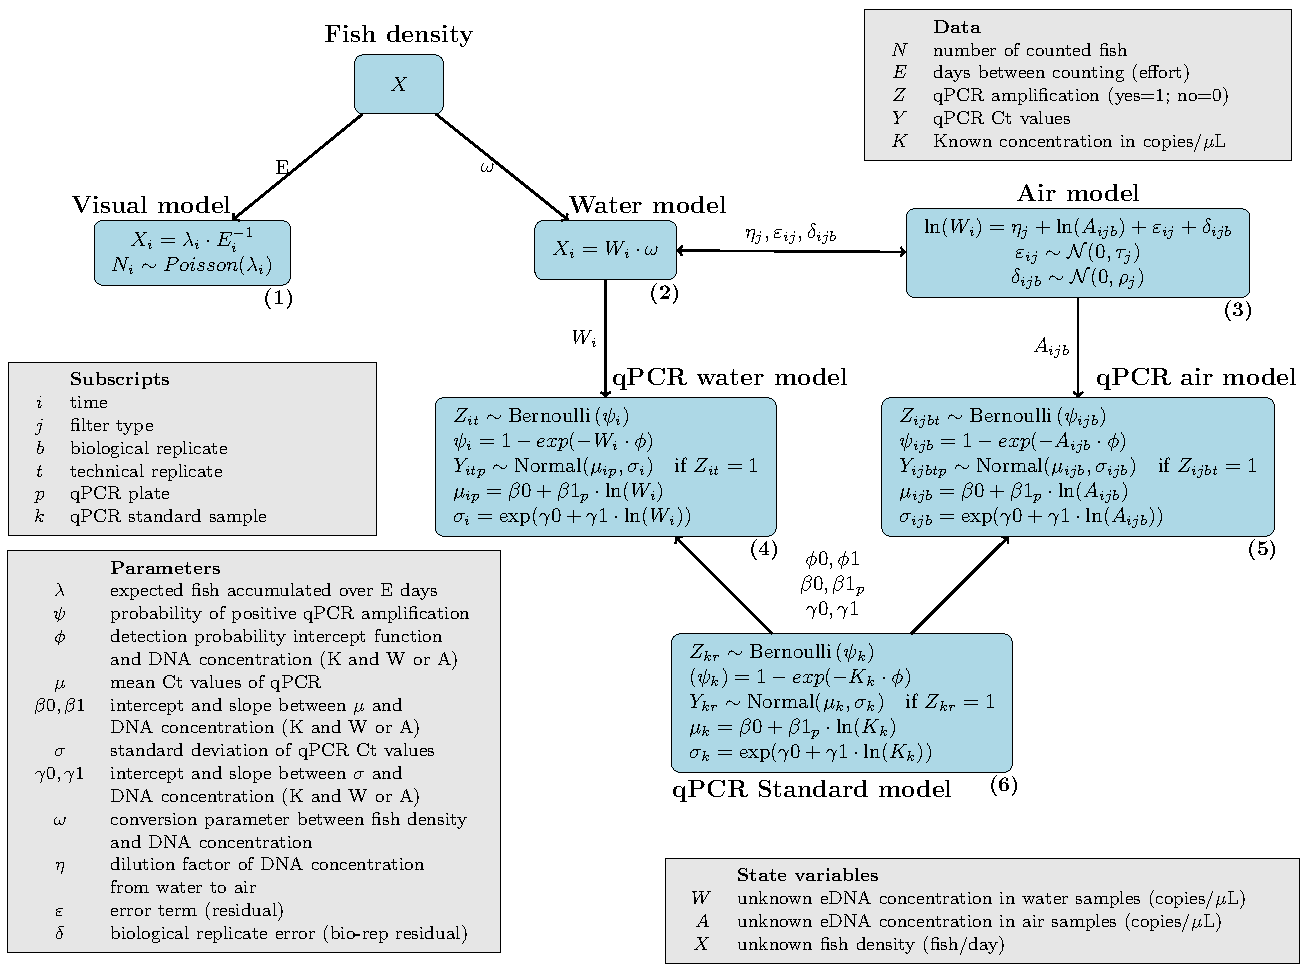
\includegraphics[width=16.5cm]{Plots/DAG.pdf}  
\caption{DAG of joint Bayesian model for estimating the eDNA concentration of Air}
\label{fig:DAG}
\end{figure}

\begin{table}[h]
    \centering
    \begin{tabular}{lll}
         & \textbf{Description} & \textbf{Prior} \\
&Data & \\
\hline
$N$ & number of fish counted & - \\
$E$ & elapsed days between counting & - \\
$Z$ & qPCR amplification (yes=1; no=0) & - \\
$Y$ & qPCR cycle threshold (Ct) & - \\
$K$ & known DNA concentration (qPCR standards) & - \\

&&\\
&State processes&\\
\hline
$X$ & unknown fish density in (fish $\cdot$ day$^{-1}$) & $\Gamma(10,1)$ \\
$W$ & unknown DNA concentration in water in (copies/$\mu$L) & - \\
$A$ & unknown DNA concentration in air in (copies/$\mu$L) & - \\
&&\\

&Transformed parameters&\\
\hline
$\lambda$& expected fish accumulated over E days & - \\
$\psi$& probability of positive qPCR amplification & - \\
$\mu$& mean Ct values of qPCR & - \\
$\sigma$& standard deviation of qPCR Ct values & - \\
&&\\

&Parameters&\\
\hline
$\omega$& conversion parameter between fish density
and DNA concentration & $\mathcal{N}(0,1)$\\
$\eta$& dilution factor of DNA concentration
from water to air & $\mathcal{N}(0,5)$\\
$\varepsilon$& time ($i$) specific error term (residual) & $\mathcal{N}(0,\tau)$\\
$\tau$& standard deviation of residuals & $\mathcal{TN}(0,1;0, +\infty)$\\
$\delta$& biological replicate error term (residual) & $\mathcal{N}(0,\rho)$\\
$\rho$& standard deviation of biological replicate error & $\mathcal{TN}(0,1;0, +\infty)$\\
$\phi$& intercept of the qPCR probability of detection ($\psi$) relationship &$\mathcal{N}(-1,1)$\\
& and eDNA concentration ($K$, $W$, and $A$) \\
$\beta0$& intercept of the linear relation between the mean Ct values ($\mu$)&$\mathcal{N}(40,1)$\\
&and eDNA concentration ($K$, $W$, and $A$) & \\
$\beta1$& slope of the linear relation between the mean Ct values ($\mu$) and &$\mathcal{N}(-3,1)$\\
&eDNA concentration ($K$, $W$, and $A$)) & \\
$\gamma0$& intercept of the linear relation between the standard deviation&$\mathcal{N}(1,0.1)$\\
&of Ct values ($\sigma$) and eDNA concentration ($K$, $W$, and $A$) & \\
$\gamma1$& intercept of the linear relation between the standard deviation &$\mathcal{N}(0,0.1)$\\
&of Ct values ($\sigma$) and eDNA concentration ($K$, $W$, and $A$) & \\
&&\\
&Index&\\
\hline
$i$& time (days) & -\\
$j$& filter type & -\\
$b$& biological sample replicate & -\\
$p$& qPCR plate & -\\
$k$& qPCR standard sample & -\\


    \end{tabular}
    \caption{Data, state processes, parameters, transformed parameters, and subscripts employed in the joint Bayesian model and their prior distributions}
    \label{tab:priortable}
\end{table}

\clearpage
\section{Results}
Here, we present findings from connecting multiple observation methods for quantifying the abundance of coho salmon, including visual counting, river water eDNA sampling, and air-based eDNA passive filtration from aerosolized particles.

\subsection{Fish accumulation based on visual counts and eDNA in river water}
At first glance, time series data revealed that coho salmon migration occurs not as a single continuous event, but rather as a series of distinct burst peaks from mid-October through late November, where the peaks are highly likely to be connected with environmental factors such as water temperature and discharge. The average daily accumulation rate (X; black line in Figure \ref{fig:fig1}) was estimated at 133.7 fish/day with peaks exceeding up to 289 fish/day and low activity of ca. 35 fish/day (Figure \ref{fig:fig1}).

%Both observation methods (river water and visual observation) are a draw from the daily accumulation rate (X), the concordance between the two abundances was revealed on the robustness of the parameter $\omega$ = 7.35 (6.99 and 7.73 lower and upper 95\% quantile) indicating that the accumulation of 1 fish/day would equal $\approx 1500$ ($\pm 500$) copies/$\mu$L reaction.

Because both observation methods (river water eDNA and visual observation) are jointly used to estimate the daily accumulation rate (X), their concordance was best evaluated through the parameter $\omega$. A converged and narrowly distributed $\omega$ parameter indicates strong agreement between the two methods and simultaneously a reliable conversion parameter from fish/day to eDNA copies/$\mu$L. In this case, $\omega$ = 7.35 (95\% quantile range of 6.99 to 7.73), suggesting consistent concordance between observed fish counts and eDNA concentrations hence, biologically, this implies that an accumulation rate of 1 fish/day corresponds to approximately 1500 ($\pm$ 500) copies/$\mu$L per reaction.

\begin{figure}[tbhp] 
\centering
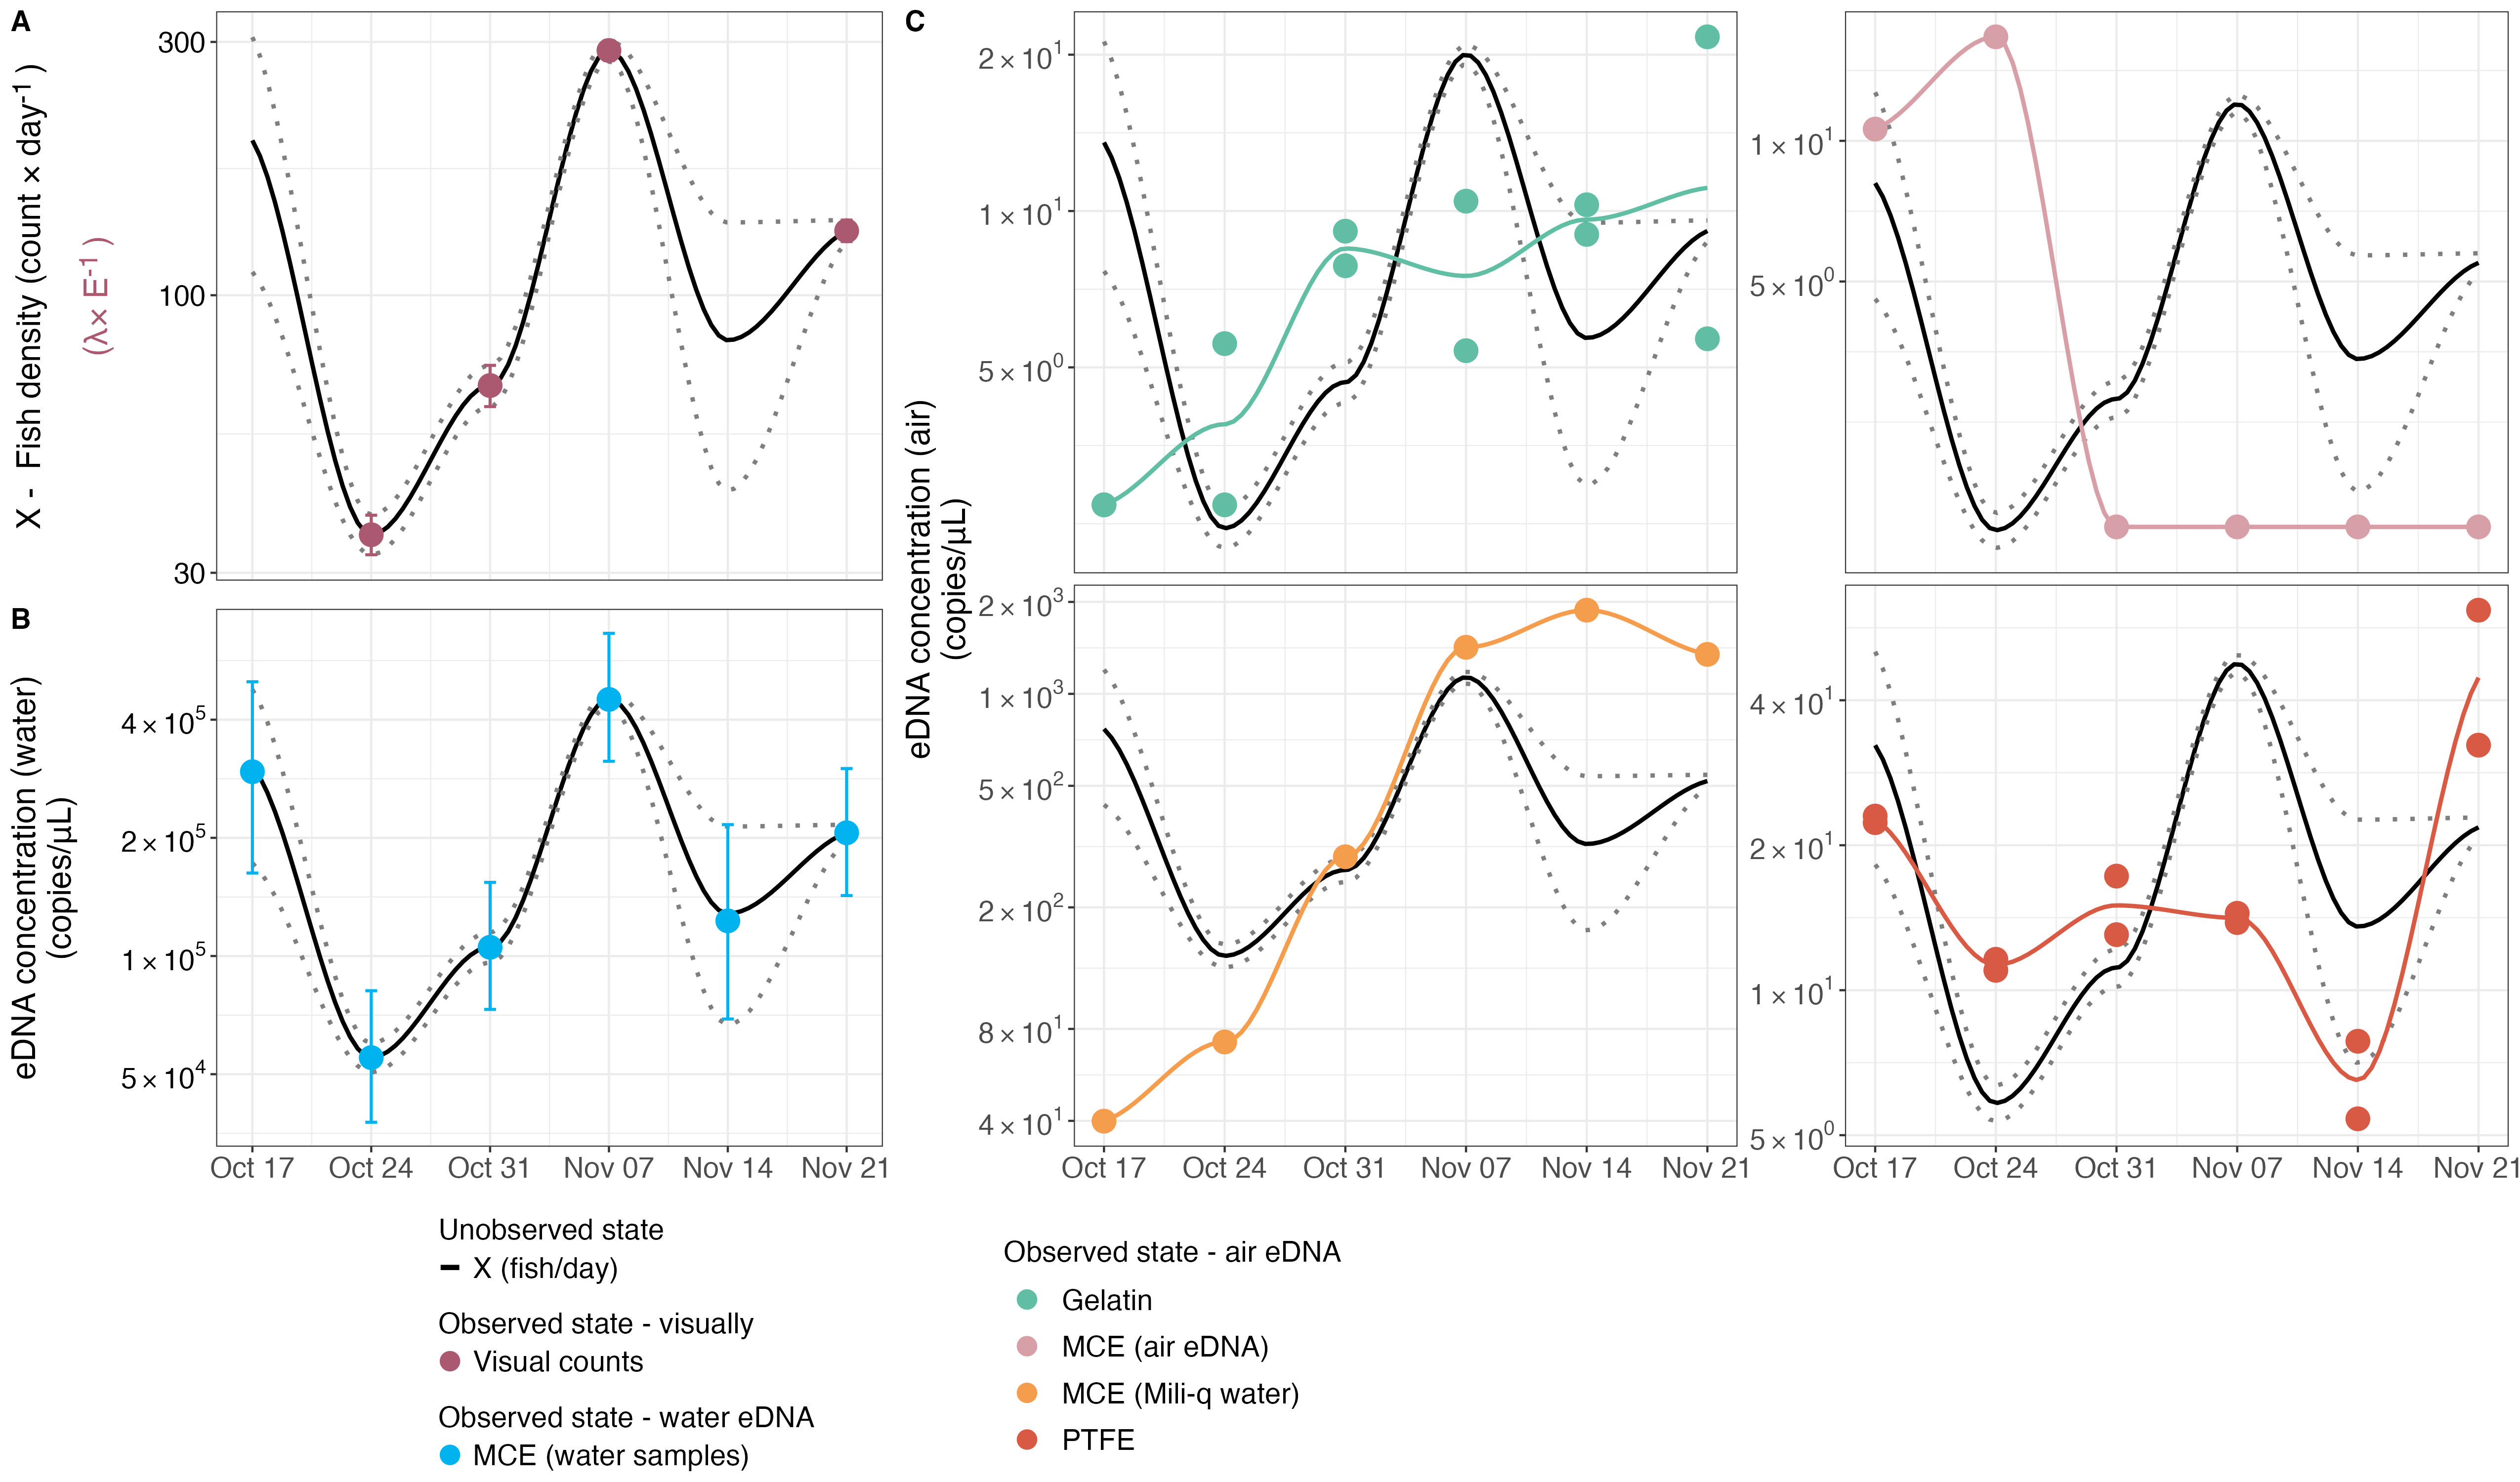
\includegraphics[width=16.5cm]{Plots/Figure_1.jpg}  
\caption{The temporal dynamics of estimated fish density in units of fish/day (X; black line with 95 confidence intervals - dotted lines) from October 17$^{th}$ to November 21$^{st}$ compared to the posterior distributions of visual observations (A), eDNA concentrations in water (B), and eDNA concentrations in air using various filter types (C).}
\label{fig:fig1}
\end{figure}


\subsection{Air eDNA signals}
Airborne eDNA originating from coho salmon was successfully detected across all passive air collection methods deployed (gelatin, PTFE, MCE filters suspended in air, and open containers of deionized water - MCE DI water). These results provide compelling proof-of-concept evidence that genetic material from aquatic organisms can be recovered from the atmosphere without requiring active airflow systems, thereby demonstrating the viability of fully passive sampling approaches for detecting airborne aquatic eDNA under field conditions.

Although all air sampling methods successfully detected the presence of upstream migratory coho salmon, we observed significant differences in recovery efficiency among filter types (Table \ref{tab:filter_error}). The airborne eDNA was recovered at varying quantities through different collection methods, with the highest recovery observed in the open containers filled with deionized water (MCE DI water), where eDNA concentrations were approximately 5.3-fold diluted compared to those measured directly in river water samples.

In contrast, suspended filters exhibited substantially lower eDNA concentrations, hence higher dilution factors: PTFE showed approximately 8.4-fold dilution, gelatin showed 9.3-fold dilution, and MCE air demonstrated the highest dilution at 9.8-fold. These differences in dilution factors reflect the varying capacities and efficiencies of different collection methods in capturing and retaining airborne aquatic eDNA from the environment.

In terms of alignment with the biological activity, PTFE and gelatin filters best mirrored the daily fish accumulation patterns, exhibiting the lowest residual errors ($\varepsilon$ = 0.570 and 0.788, respectively).  Conversely, MCE DI water, despite recovering the highest eDNA concentration, showed less parsimony with the fish migration dynamics ($\varepsilon$ = 0.974; Figure \ref{fig:fig1}). The MCE air suspended filters performed least effectively in tracking temporal migration patterns, failing to amplify coho salmon DNA beyond the first two weeks of the sampling campaign.

Subsequently, biological replicates for gelatin and PTFE filters revealed additional insights regarding methodological robustness and reproducibility. PTFE filters produced the most consistent quantifications, with lower variance between replicates ($\delta$ = 0.106), whereas gelatin filters showed a higher degree of variability ($\delta$ = 0.230), indicating reduced reproducibility of quantitative outcomes. 

These findings underscore the importance of filter selection in both the sensitivity and reliability of airborne eDNA monitoring.

\begin{table}[h!]
\centering
\caption{Error measurements for different filter types}
\label{tab:filter_error}

\begin{tabular}{llll}
\textbf{Filter type} & \textbf{Dilution ($\eta$)} & \textbf{Error ($\overline{|\varepsilon|}$)} & \textbf{Biological rep error ($\overline{|\delta|}$)} \\
Gelatin & $e^{-9.25}$ & 0.788 & 0.230 \\
PTFE & $e^{-8.39}$ & 0.570 & 0.106 \\
MCE Air & $e^{-9.77}$ & 1.370 & - \\
MCE DI water & $e^{-5.33}$ & 0.974 & - \\
\end{tabular}
\end{table}


\subsection{Model diagnostics}

Convergence and reliability of the Bayesian model were assessed through comprehensive diagnostics. All parameters (Table \ref{tab:priortable}) exhibited Gelman-Rubin convergence statistics ($\hat{R} < 1.01$) and effective
sample sizes (ESS) exceeding 1000 per parameter, indicating successful convergence and efficient mixing of
the six independent chains (Figure \ref{fig:diagnostics}\textit{A}). 


No divergent transitions were detected during sampling, and the maximum tree depth was not exceeded, indicating no issues with divergence or exploration limits (Figure \ref{fig:diagnostics}\textit{B}). The posterior likelihood demonstrated convergence before the sampling phase began, with all chains exhibiting high mixing, confirming robust exploration of the parameter space (Figure \ref{fig:diagnostics}\textit{B}).

Prior sensitivity analyses revealed that posterior estimates differed from priors, demonstrating that the posteriors were appropriately updated based on the observed data rather than being heavily influenced by prior assumptions (Figure \ref{fig:prior_sens}). Additionally, the posterior predictive checks (PPC) demonstrated that the model reliably reproduced the observed data, supporting the validity of parameter estimates (Figure\ref{fig:prior_sens}). 

Collectively, these diagnostics confirm the reliability and validity of the Bayesian model used here.

\begin{figure}[tbhp] 
\centering
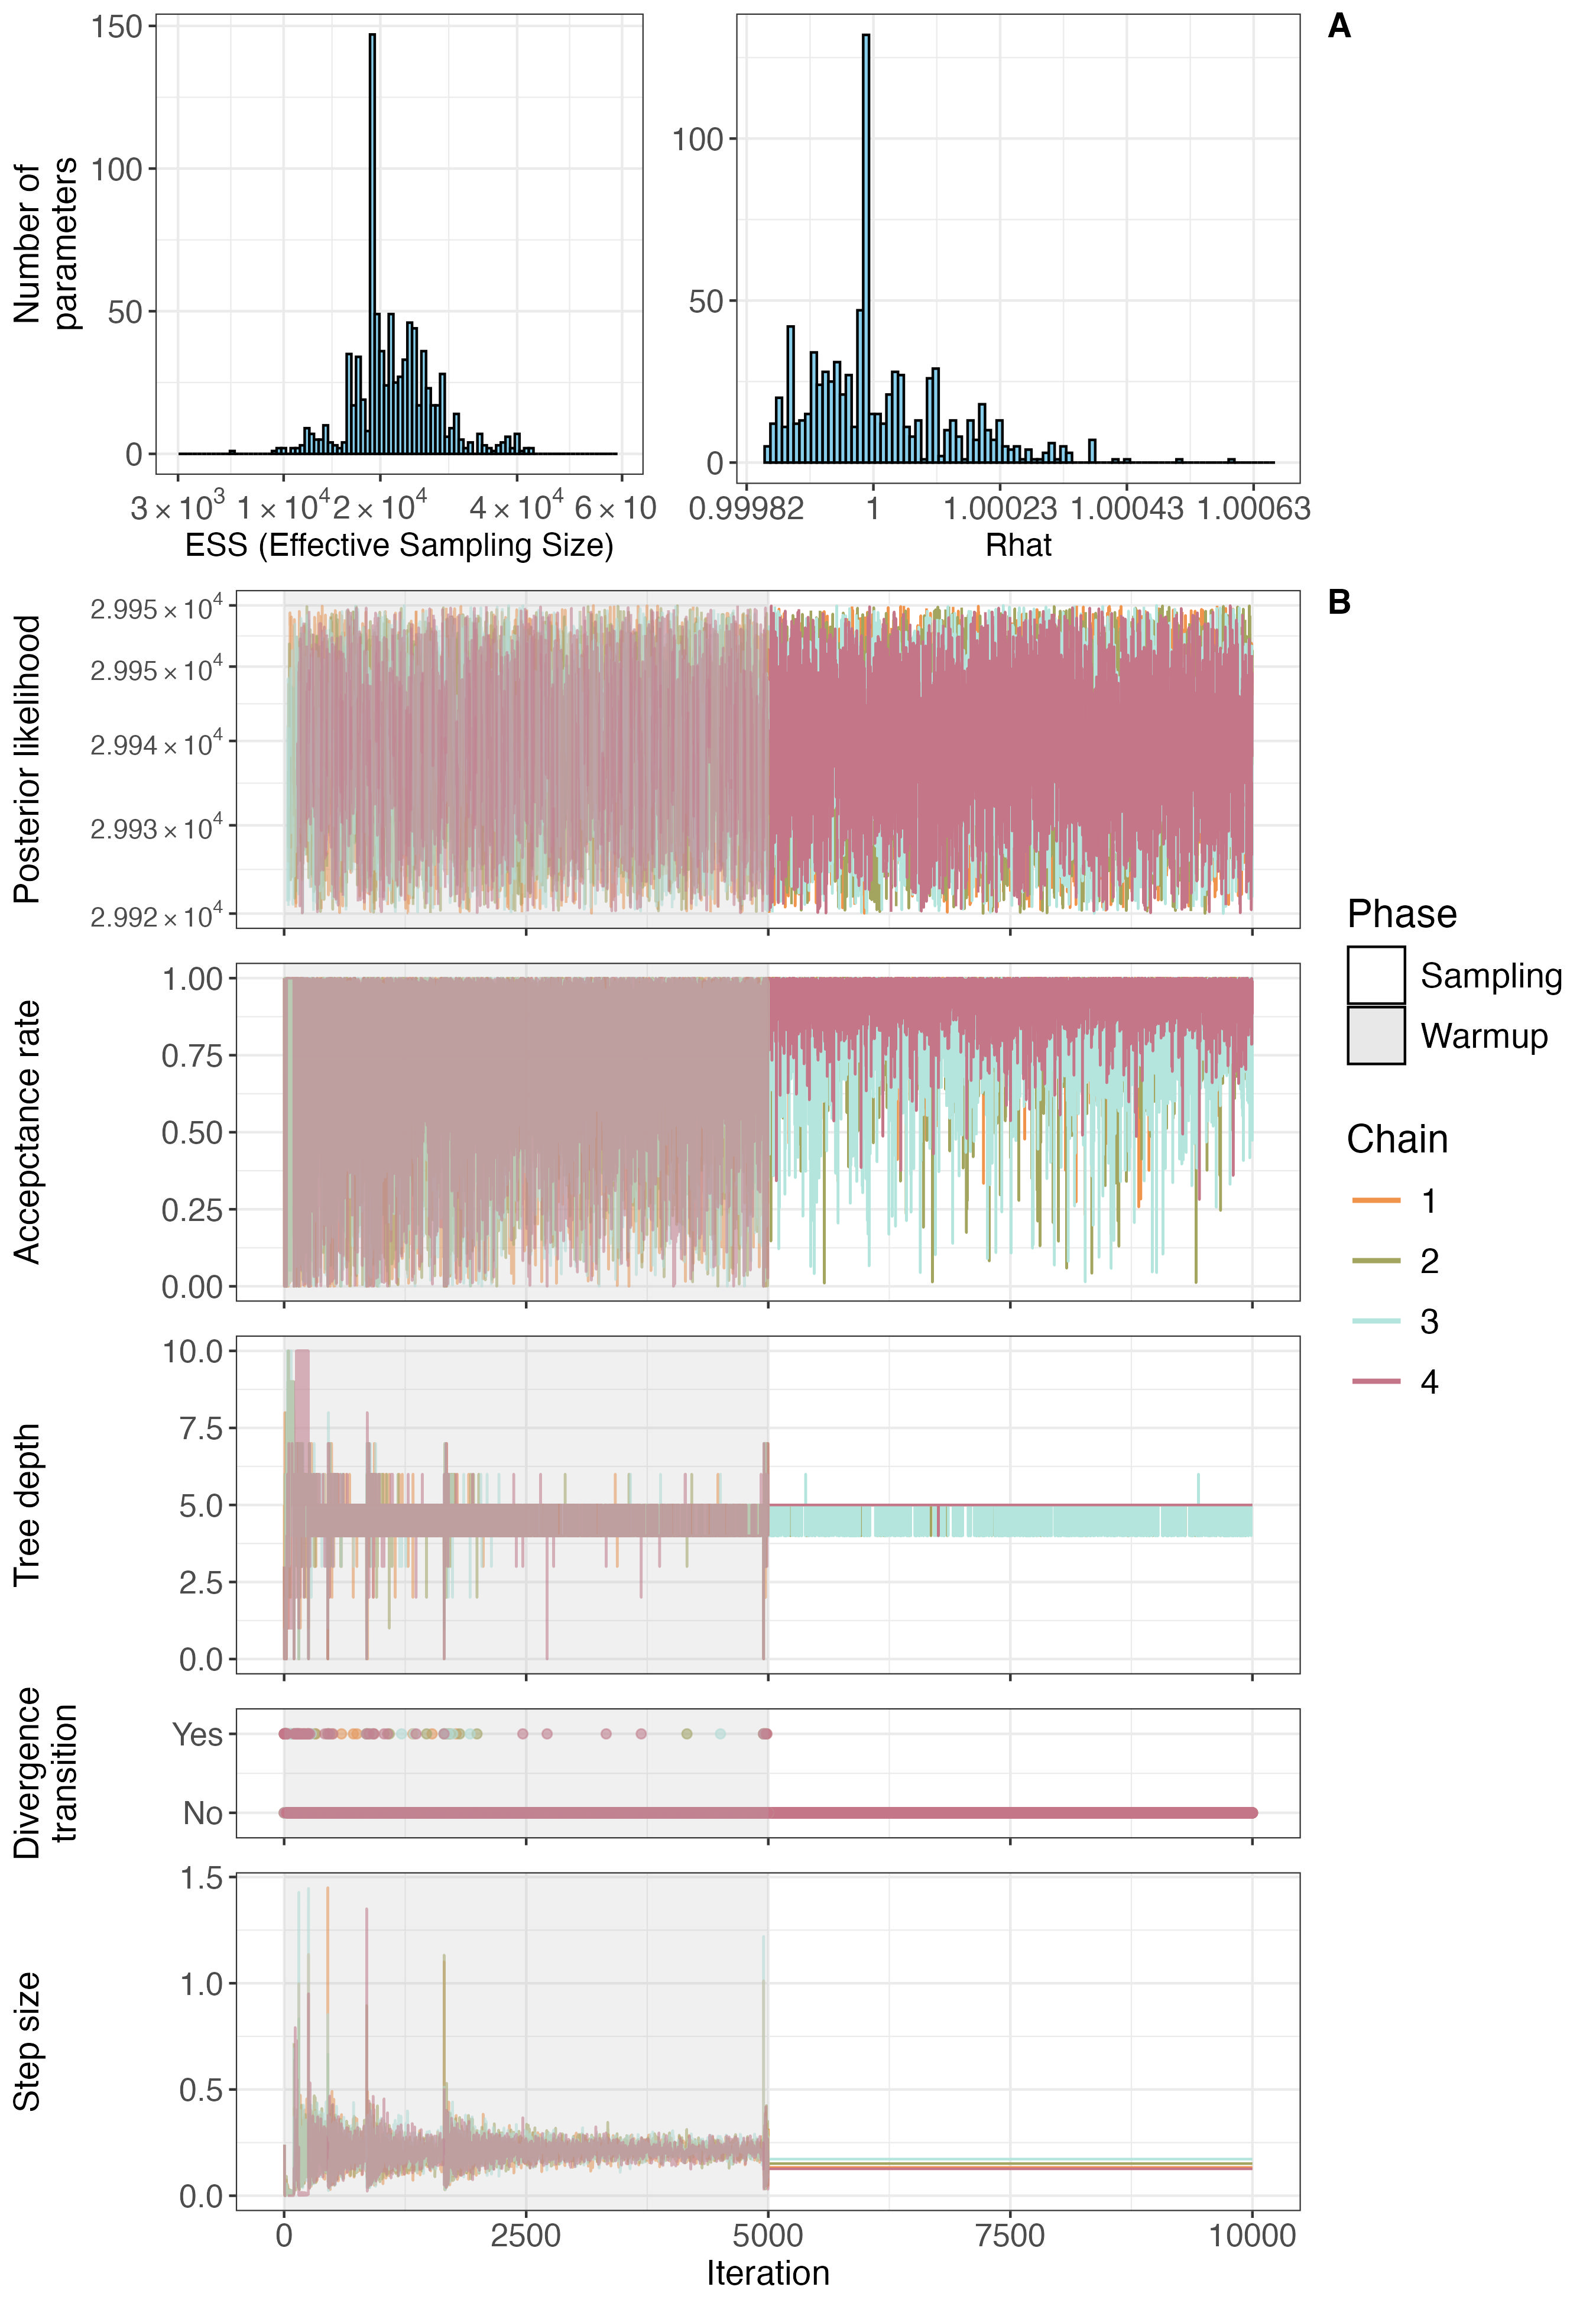
\includegraphics[width=16.5cm]{Plots/Diagnostic_Fig_1.jpg}  
\caption{Model diagnostics}
\label{fig:diagnostics}
\end{figure}


\begin{figure}[tbhp] 
\centering
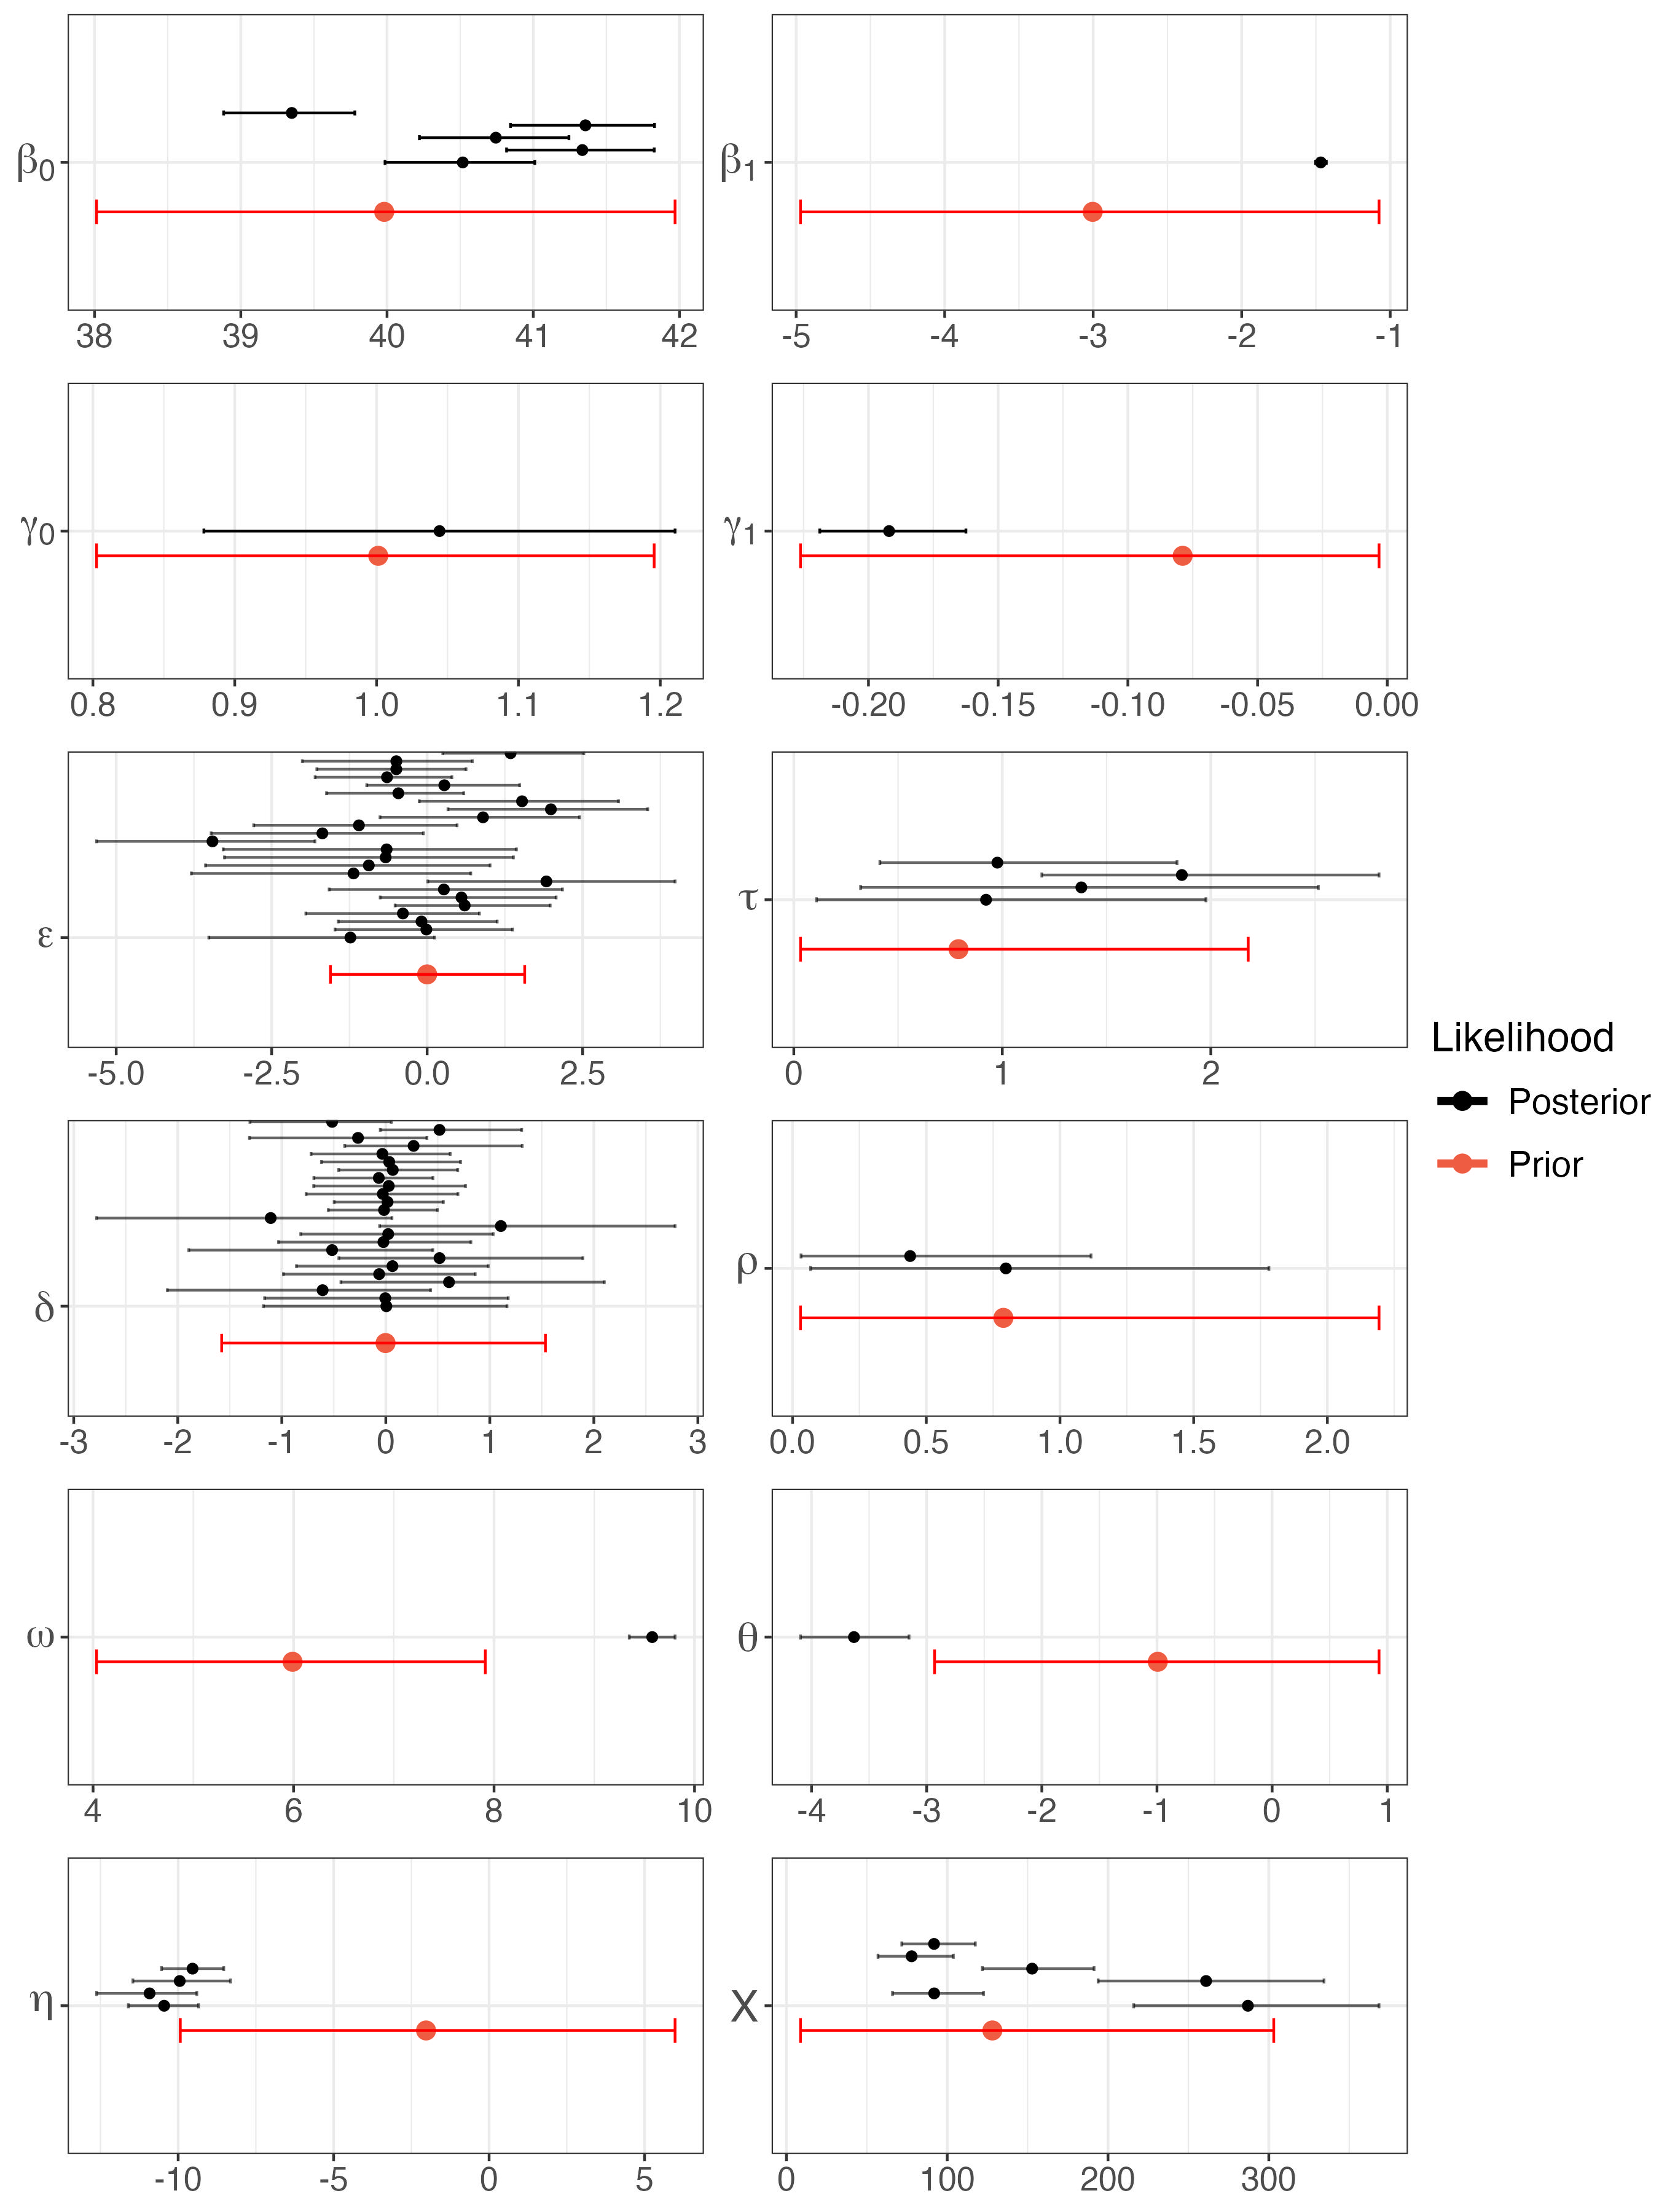
\includegraphics[width=16.5cm]{Plots/Diagnostic_Fig_2.jpg}  
\caption{Prior sensitivity analysis}
\label{fig:prior_sens}
\end{figure}

\section{Discussion}
Our study establishes, for the first time, that passive airborne eDNA sampling can reliably capture and quantify molecular signals from aquatic organisms. This represents a paradigm shift in how we access aquatic biodiversity—through the air, without ever touching the water. In salmon-spawning streams, genetic material from the river is transported into the air likely by evaporation, bubble-burst aerosolization at riffles and splashes, and the rigorous churning of spawning fish (Wood et al., 2021; Prather et al., 2013). Collections from multiple passive samplers, when compared with conventional water-based eDNA assays and daily visual counts, reveal a clear and quantitative relationship between airborne eDNA concentration and salmon density. 

Until now, airborne eDNA surveys have reported fish or other strictly aquatic taxa as likely to be laboratory contamination, zoo-feed artifacts, or piscivore fecal bioaerosols (Klepke et al., 2022; Lyngaard et al., 2022; Lyngaard et al., 2023; Sullivan et al., 2023). Our data suggest otherwise: this is a real ecological signal rather than an experimental artifact. It is likely that wind speed, relative humidity, and temperature will determine how far and how long aerosolized aquatic eDNA will travel before being redeposited (Abrego et al. 2024; Giolai et al., 2024). For example, high humidity and rainfall force rapid settling and very localized deposition while dry, windy conditions might carry genetic plumes further distances downwind (Galbán et al., 2021; Maki et al., 2023). These environmental controls, combined with air currents above riffles and splashes, should be considered when determining how passive samplers capture transient pulses of biological activity.



HEADER -- SOMETHING ABOUT DILUTION AND DURATION OF PASSIVE AIR SAMPLING METHODS 
On average, our data showed that eDNA in the air was 10 billion times less concentrated than in the water, yet these dilute signals remain faithful indicators of fish presence and population density. Although airborne eDNA yields are low, our sensitive laboratory methods and rigorous statistical models detected unambiguous, quantitative patterns. EXPAND A BIT ON DILUTION? MAYBE EXPLORE SOMETHING LIKE LIMIT OF DETECTION AND DISCUSS HOW DURATION OF AIR SAMPLING MIGHT BE AT PLAY - LIKE LONGER TIME MIGHT ACCUMULATE MORE EDNA BUT BALANCE WITH DECAY/DEGRADATION - SO FOR EXAMPLE A WEEK DEPLOYMENT OF A PASSIVE AIR SAMPLER YOU PROBABLY DON'T HAVE ANY DNA LEFT FROM DAY 1 BUT MOSTLY DNA FROM DAY 7, THEN 6, ETC.  

Our findings accord with the recent work by Jager et al. (2025) who showed that passive air samplers outperform active pumps by sampling intermittent, DNA-rich plumes over long intervals and detecting greater species richness. In our streams, passive filters similarly intercepted heterogeneous bursts of salmon eDNA without power or infrastructure while active-pump systems—limited by shorter run times and larger air-volume draws—would have averaged across plumes and risk diluting localized signals.

HEADER -- SOMETHING ABOUT ORIENTATION AND FILTER MATERIAL PROPERTIES OF PASSIVE SAMPLING METHODS
Over 24-hour deployments, vertically oriented gelatin and PTFE filters acted as higher-resolution “fish-activity” samplers (Jager et al., 2025). Ambient air currents likely swept fine, splash-generated aerosols rich in salmon DNA onto their membranes, producing yields that rose and fell in accordance with live fish counts and water-eDNA levels (Blanchard et al., 1980). In contrast, the large horizontal tray of deionized water seemed to function more like a hydraulic-driven deposition trap. The container saw a steady accumulation of eDNA over the six weeks and thus could have been collecting more coarse spray, foam, and decay-derived particulates from river turbulence and from decomposing carcasses (Prather et al. 2013; Hinds 1999). Because salmon carcasses often remain in shallow banks and backwaters as the spawning season progresses, it is plausible that river turbulence and discharge could generate larger droplets over decomposing tissue, potentially facilitating eDNA dispersal (Wood et al., 2021; Herman, 2023). These coarse droplets settle rapidly and dominate deposition on horizontal collectors while the fine fraction produced by active fish movement is under-represented. Gelatin and PTFE filters thus seem to provide snapshots of biologically driven eDNA flux whereas the water tray seemed to integrate both flow-driven and decay-driven inputs into a monotonic accumulation curve.

The filter materials and operational context also likely affected the air sampling performance. In terms of filter materials, PTFE filters, known for their durability, delivered the most consistent results of all the passive filtration methods; gelatin filters yielded the highest sensitivity but showed greater variability; mixed cellulose ester filters captured negligible airborne DNA; and the open tray, with roughly 50 times more surface area than the vertical filters, recovered the highest total DNA yield. The different passive sampling methods also are affected differently by operational contexts such as weather. For the filters, PTFE and MCE should be unaffected by rain, however the gelatin filters perform better under dry conditions as they dissolve when wet. For the tray, rain can dilute the water sample, but the larger surface area and direct water input from rain can also increase DNA capture but demand extra processing. Future work should XXX look at weather or something to that effect. 

HEADER - SOMETHING ABOUT POTENTIAL ADVANTAGES AND LIMITATIONS 
Perhaps most striking result from our work is the simplicity and versatility of passive airborne sampling. No pumps or power are needed, and equipment is extremely low cost and easy to deploy. This minimal-infrastructure approach makes it viable for remote headwaters, steep mountain channels, urban stormwater networks, and contaminated ponds where water sampling is unsafe (Harrison et al., 2019; Bagley et al., 2019). By integrating visual surveys, water-based eDNA and airborne eDNA, we establish a biomonitoring framework that is non-invasive, scalable and low-impact. In an era of intensifying droughts, floods and public-health risks such as bacterial outbreaks in stagnant waters, airborne eDNA offers resilient pathways for rapid invasive-species alerts, real-time disease surveillance in flood-prone wetlands and non-invasive population censuses in protected spawning grounds.

Naturally, challenges remain. Passive deployments rely on surface-area-by-time metrics rather than standardized air-volume units, complicating direct comparisons across studies. Optimal exposure times must balance accumulation against DNA degradation from UV, microbes and moisture (Brandáo-Dias et al., 2023). Weather variability in wind, humidity and rain can alter deposition rates and sampler efficiency (Johnson et al., 2023; Johnson et al., 2024). Future work should refine sampler design, systematically compare vertical and horizontal orientations, explore automated or drone-based retrieval and integrate river discharge and meteorological data into quantitative models (Galbán et al., 2021; Kirchgeorg et al., 2024; Shogren et al., 2017; Wood et al., 2021).

Our study begins to chart a portion of airborne eDNA ecology's in five key dimensions (Johnson et al., 2024). We confirm origin by matching airborne DNA trends to co-occurring water eDNA and fish counts. We elucidate transport mechanisms such as evaporation, bubble bursts and fish activity. We quantify dispersal and dilution by measuring a 10-billion-fold concentration difference between water and air samples. We demonstrate fate through differential deposition on vertical filters and horizontal trays. Finally, we show that airborne DNA fragments remain amplifiable, offering an initial glimpse into their molecular state after transport. These insights lay the groundwork for future studies on persistence, degradation and particle-size distributions from airborne eDNA (Brandão-Dias et al., 2023; 2025).

Overall, our work overturns the assumption that aquatic eDNA belongs solely underwater. By demonstrating that genetic signals from fish and other aquatic life routinely escape into and can be captured from the air, we open a new paradigm for ecological monitoring. The atmosphere above water emerges as a reliable, quantifiable reservoir of biodiversity data. This advance promises transformative applications from invasive species alerts in drought-stricken reservoirs to pathogen surveillance in flood-prone wetlands and non-invasive censuses in protected streams, equipping managers with a resilient, real-time window into aquatic ecosystems.

\section*{Acknowledgments}
We thank Natasha Kacoroski, Larry Franks, and the dedicated volunteers at Friends of the Issaquah Salmon Hatchery for their generous support in the field. We are also grateful to Travis A. Burnett and Darin Combs at the Washington Department of Fish and Wildlife for facilitating access and permitting field experimental work at the Issaquah Hatchery. Additional thanks to Pedro F.P. Brandão-Dias for assistance with air filter deployments, and to Kevan Yamanaka at the Monterey Bay Aquarium Research Institute for designing and fabricating the 3D-printed passive filter holders. We are especially grateful to Chris Sergeant for valuable insights on salmon biology that shaped the interpretation of our findings, and to Ole Shelton for statistical advice that improved our analytical approach. We acknowledge funding support from the Packard Foundation [Grant No. GR016745] and thank the Center of Environmental Genomics for providing access to high-performance computing resources.

\section*{Author contributions}
Y.C.A.I. conceived the study. Y.C.A.I. G.G and E.A.A. designed the field and laboratory protocols. Y.C.A.I. and G.G. jointly designed the downstream statistical analyses and Bayesian modeling framework. G.G. conducted all statistical analyses, with inputs from R.P.K. The fieldwork was performed by Y.C.A.I. and E.A.A., while Y.C.A.I. and G.G. co-wrote the manuscript. R.P.K. supervised the project, contributed to conceptual guidance, and provided critical revisions. All authors contributed to the study design and approved the final manuscript.  

\section*{Data availability}
The authors declare that they have no competing interests. All data needed to evaluate the conclusions in this paper are available in the main text and/or the Supplementary Materials. Additional data, code, and materials will be made available upon reasonable request. No materials were subject to material transfer agreements (MTAs).

\clearpage
\bibliography{Bib.bib}
\end{document}


\begin{table}[h]
    \centering
    \begin{tabular}{llll}
        \textbf{Filter type} & \textbf{Dilution ($\eta$)} & \textbf{Error ($\overline\varepsilon$)} & \textbf{Biological rep error ($\overline\delta$)} \\
        Gelatin & $e^{-9.5}$ & 0.628 & 1.315 \\
        PTFE & $e^{-8.8}$ & 0.666 & 0.682 \\
        MCE air filter & $e^{-10.2}$ & 1.133 & - \\
        DI water & $e^{-5.7}$ & 0.606 & - \\
    \end{tabular}
    \caption{Error measurements for different filter types}
    \label{tab:filter_error}
\end{table}



Fish Density Model (Water): The number of fish counted ('N') at a given point is assumed to be proportional to the total amount of water-borne DNA, which can be estimated from measurements taken underwater and converted into an 'eDNA concentration' parameter ('W'). This conversion process involves multiplying by another factor called 'omega', denoted as 'ω'.
Air Model: The eDNA concentrations in air samples are calculated based on those found in the corresponding water sample using a dilution factor, which is determined from measurements taken underwater and above ground (i.e., atmospheric pressure). These factors include both known ('K') and unknown values of DNA concentration that need to be estimated during model fitting or inference processes.
qPCR Model: The number of positive amplification results in the various types of samples are assumed to follow a Poisson distribution, with mean proportional to their respective eDNA concentrations (W for water-borne species) as well as effort ('E', which represents days between counting). This relationship is captured by parameters like 'phi0' and 'phi1'.
Visual Model: The probability of finding fish in an underwater visual census survey follows a logistic model, with the logit link being determined by linear combinations involving eDNA concentration (W) as well as other covariates ('X') such as depth or temperature measurements taken at each counting event. This relationship is represented by parameters like 'beta0' and 'beta1'.
Standard Model: In cases where a known standard sample with DNA content of K copies/μL exists, the model allows for estimation of eDNA concentrations in water samples ('W') using this reference value as well as other covariates (X). The relationship is determined by parameters like 'gamma0' and 'gamma1'.
Error Terms: Various error terms are included to account for uncertainty or variability introduced during different stages of the analysis process, such as biological replicates in air sampling ('delta b'), residuals from model equations involving eDNA concentration (omega), dilution factors between water-borne vs atmospheric DNA samples (eta) and technical replicate measurements taken within each type of sample. By incorporating these relationships into a single graphical structure that can be analyzed using statistical software, researchers are able to estimate parameters like 'W', 'A' or other key ecological variables with improved accuracy compared to traditional methods relying solely on one specific analytical technique alone (e.g., qPCR).

We can start by defining λ as fish density, where ω represents a conversion parameter from fish/day to copies/μL (the unit for DNA concentrations). This means that W = λ * ω and $A_b = η^(-1)$ / B. The air model also includes the δ error term representing biological replicate differences between samples taken at different times or using different filters, leading to a final equation of:
Aij= (ηj + ln(PB))/B with PB being an unknown constant that depends on both filter type and bioreplicate difference in time. The qPCR water model can be defined similarly as $Z = ψ_i * W^(-1)$ where μ is the mean Ct values of a standard curve, β represents slopes between DNA concentration (K or A), σ being its corresponding error term for each sample i at different times t during counting and plate p. The qPCR air model can be defined as $Z = ψ_k * K^(-1)$ with μ representing the mean Ct values of a standard curve, β represents slopes between DNA concentration (K or A), σ being its corresponding error term for each sample i at different times t during counting and plate p. The qPCR Standard model can be defined as $Z = ψ_i * W^(-1)$ with φ representing intercepts/slopes of the probability response to standard curve concentrations K, μ mean Ct values from a single amplification cycle (Ct), σ being its corresponding error term for each sample i at different times t during counting and plate p. The parameters can be estimated using maximum likelihood estimation or Bayesian methods such as MCMC sampling if needed given prior distributions specified on all unknown quantities including $W_i = η^(-1) / B$ with PB representing an unknown constant that depends both filter type bioreplicate difference in time, ε error term (residual), and δ being biological replicate errors. The subscripts provide information about the variables at different times i during counting or using filters jb for each sample b taken over multiple plates pqPCR standard samples k
